\documentclass{article}

% Code syntax highlighting
% https://www.overleaf.com/learn/latex/Code_Highlighting_with_minted
\usepackage{minted}
\usemintedstyle{borland}

% If you're new to LaTeX, here's some short tutorials:
% https://www.overleaf.com/learn/latex/Learn_LaTeX_in_30_minutes
% https://en.wikibooks.org/wiki/LaTeX/Basics

% Formatting
\usepackage[utf8]{inputenc}
\usepackage[a4paper, margin=1in]{geometry}
\usepackage[titletoc,title]{appendix}
\usepackage{indentfirst}

% Math
% https://www.overleaf.com/learn/latex/Mathematical_expressions
% https://en.wikibooks.org/wiki/LaTeX/Mathematics
\usepackage{amsmath,amsfonts,amssymb,mathtools}
\DeclareMathOperator*{\argmax}{argmax} % thin space, limits underneath in displays


% Images
% https://www.overleaf.com/learn/latex/Inserting_Images
% https://en.wikibooks.org/wiki/LaTeX/Floats,_Figures_and_Captions
\usepackage{graphicx,float}
%Path relative to the main .tex file 
\graphicspath{ {./images/} }

% Tables
% https://www.overleaf.com/learn/latex/Tables
% https://en.wikibooks.org/wiki/LaTeX/Tables

% Algorithms
% https://www.overleaf.com/learn/latex/algorithms
% https://en.wikibooks.org/wiki/LaTeX/Algorithms
\usepackage[ruled,vlined]{algorithm2e}
\usepackage{algorithmic}


% Sections in a new page
\usepackage{titlesec}
\newcommand{\sectionbreak}{\clearpage}
% \newcommand{\subsectionbreak}{\clearpage}

\usepackage{hyperref}

\usepackage{tabularx}


% Title content
\title{A0184594N}
\author{A0184594N}

\begin{document}

\section{Chapter 3 - Parallel Computing Platforms}

\subsection{Source of Processor Performance Gain}
Parallelism of various forms exist to have some performance gain
\begin{itemize}
    \item Single Processor
          \begin{itemize}
              \item Bit Level
                    \begin{itemize}
                        \item We don't processs bit by bit, but instead word by word.
                    \end{itemize}

              \item Instruction Level
                    \begin{itemize}
                        \item Pipelining (parallelism across time)
                              \begin{itemize}
                                  \item Split instruction into different stages
                                  \item allow multiple instructions to occupy different stages at same clock cycle.
                                  \item Number of pipeline stages == Maximum achievable speedup
                              \end{itemize}
                        \item Superscalar (parallelism across space)
                              \begin{itemize}
                                  \item Duplicate the pipelines
                                  \item Allow multiple instructions to pass through the same stage.
                                  \item Hard to schedule, find instructions that can be run together. (Dymanic - Hardware decision, Static - Compiler decision)
                                  \item Disadvantage: structural hazard
                              \end{itemize}
                        \item But is very limited, at most 2-3 instructions one time. due to data/control dependencies
                        \item Most CPUs have this. Usually we calculate Instructions per cycle, not Cycle-per-instruction.
                    \end{itemize}
              \item Thread Level
                    \begin{itemize}
                        \item Multithreading was originally a software mechanism
                        \item allow multiple parts of the same program to execute concurrently
                        \item Processor can provide hardware support for "thread context" like program counter and register (hyper-threading, etc..)
                        \item software threads can be executed in parallel
                    \end{itemize}
                    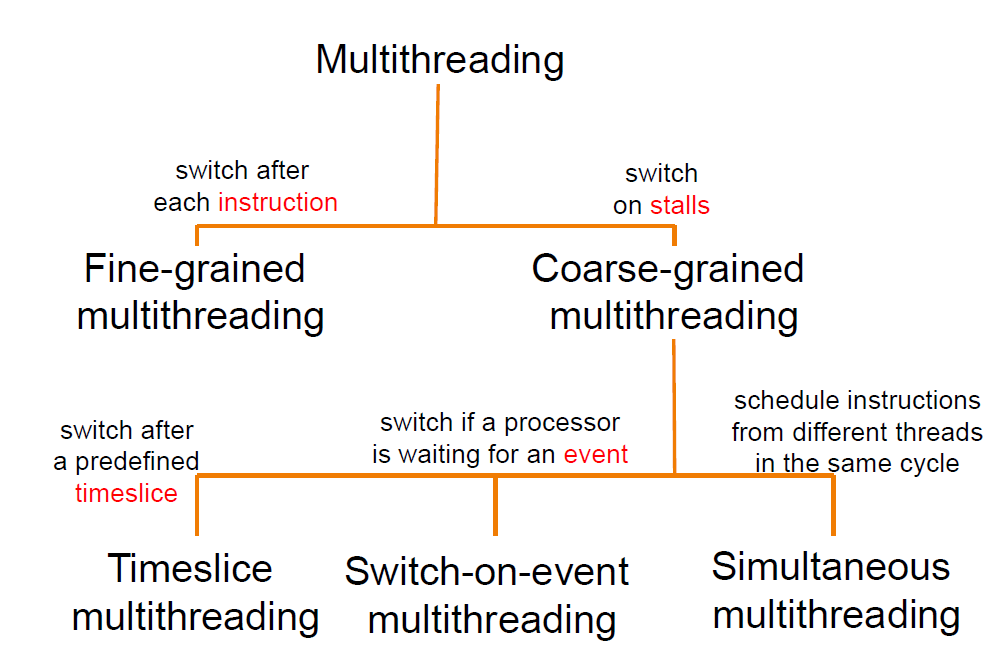
\includegraphics[width=0.7\textwidth]{l3_multithreading_implementation}
              \item Process Level
                    \begin{itemize}
                        \item Multiple processes work in parallel
                        \item independent memorry space, need special mechanism to communicate
                        \item Operating system provide IPC (Inter-Process communication) mechanism
                        \item Each process has independent context, can be mapped to multiple processor cores
                    \end{itemize}
          \end{itemize}
    \item Multi Processor
          \begin{itemize}
              \item Processor Level
                    \begin{itemize}
                        \item Shared Memory
                        \item Distributed Memory
                    \end{itemize}
          \end{itemize}
\end{itemize}

\subsection{Flynn's Parallel Architecture Taxonomty}
\begin{itemize}
    \item SISD (Single Instruction Single Data)
          \begin{itemize}
              \item A single instruction stream is executed
              \item Each instruction work on single data
              \item Most of the uniprocessor
          \end{itemize}
    \item SIMD (Single Instruction Multiple Data)
          \begin{itemize}
              \item A single stream of instructins
              \item Each instruction work on multiple data
              \item supercomputer during 1980s
              \item To exploit data parallelism, also known as vector processor
              \item Most modern processor has some form of SIMD
          \end{itemize}
    \item MISD (Multiple Instruction Single Data)
          \begin{itemize}
              \item Multiple stream of instructins
              \item All instruction work on same data at any time
              \item No actual implementaion, just here for completeness
          \end{itemize}
    \item MiMD (Multiple Instruction Multiple Data)
          \begin{itemize}
              \item Each Processing Unit fetch its own instruction
              \item Each Processing operates on its data
              \item Most popular model for multiprocessor
          \end{itemize}
\end{itemize}

Variant - SIMD and MIMD. nVidia GPUs have a set of threads executing the same code (SIMD) and multiple set of threads executing in parallel (MIMD)

\subsection{Multicore Architecture}
\subsubsection{Hierarchical design}
Multiple cores share multiple caches.
Cache size increase from the leaves to the root.
Found in comon day desktop, GPUs.

\subsubsection{Pipelined design}
Data elements are processed by multiple (different) execution cores in a pipelined way.
Bacuase same computation steps have to be applied to a long sequence of data elements.
Found in networking application, or GPUs.

\subsubsection{Network-based design}
Cores and their local caches and memories are connected via an interconnection network
Each core communicate with other cores / memory through this network.

\subsection{Memory Organization}
Memory can have consistency problem.
If one processor updates value in memory, How will other cores also update their values.
This also extends to the cache. Where we have cache coherence problem.
If we update value in the cache, how will other processor also update the same value in their caches.

2 Factors differentiate shared memory systems
\begin{itemize}
    \item Processor to Memory Delay (UMA/NUMA)
    \item presence of a local cache with cache coherence protocol (CC/NCC)
\end{itemize}

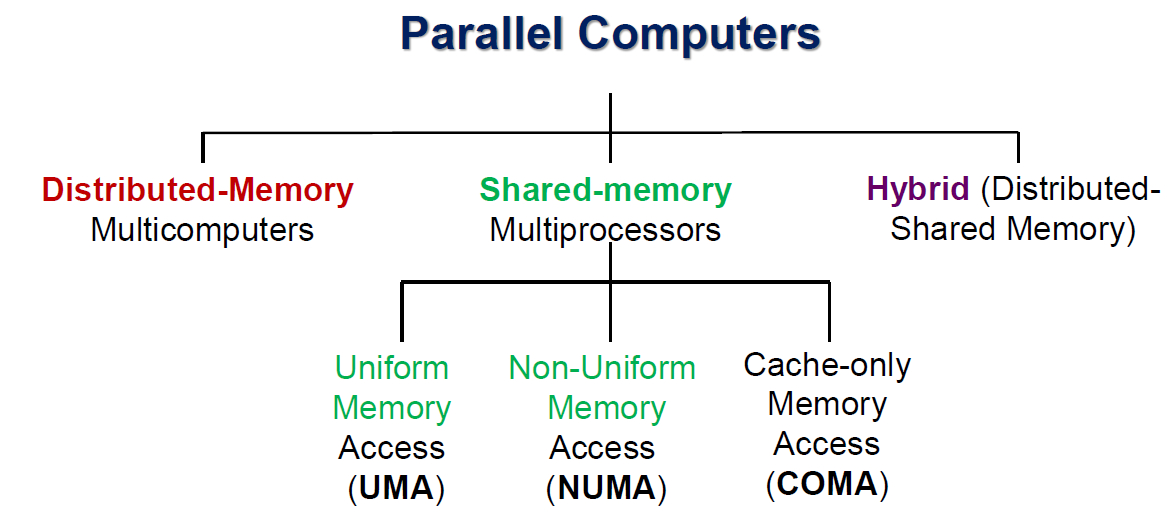
\includegraphics[width=0.9\textwidth]{l3_memory_organization}

\begin{itemize}
    \item Distributed Memory Systems
          \begin{itemize}
              \item Each node is independent, communicate with message passing
          \end{itemize}
          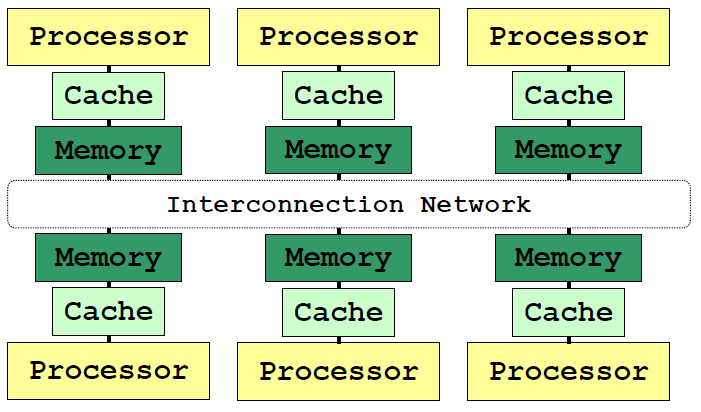
\includegraphics[width=0.9\textwidth]{l3_distributed_memory_system}
    \item Shared Memory
          \begin{itemize}
              \item Uniform Memory Access (Time) (UMA)
                    \begin{itemize}
                        \item Latency of accessing main memory is the same for each procesor
                        \item Good for low under of processors
                    \end{itemize}
                    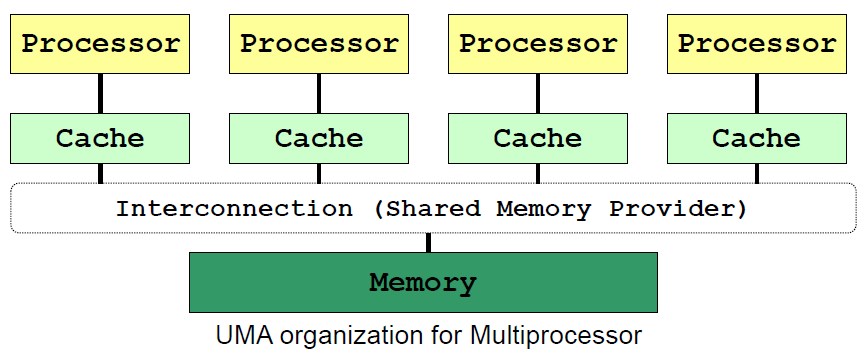
\includegraphics[width=0.9\textwidth]{l3_uniform_memory_access}
              \item Non-Uniform Memory Access
                    \begin{itemize}
                        \item Physically distributed memory of all processing elemets are combined to form a global shared memory
                        \item Processor can access local memory faster than remote memory
                    \end{itemize}
                    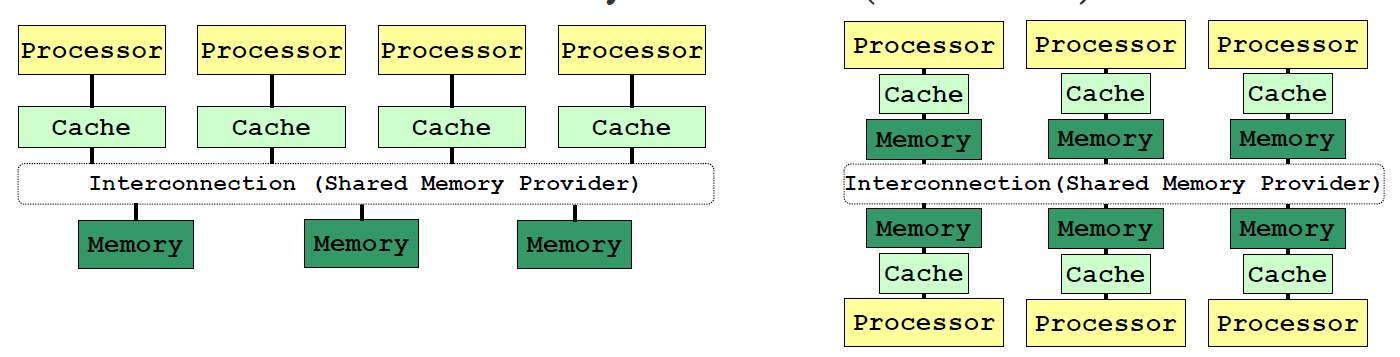
\includegraphics[width=0.9\textwidth]{l3_numa.png}
              \item Cache Coherent Non Uniform Memory Access (ccNUMA)
                    \begin{itemize}
                        \item Each node has cache to reduce contention
                    \end{itemize}
                    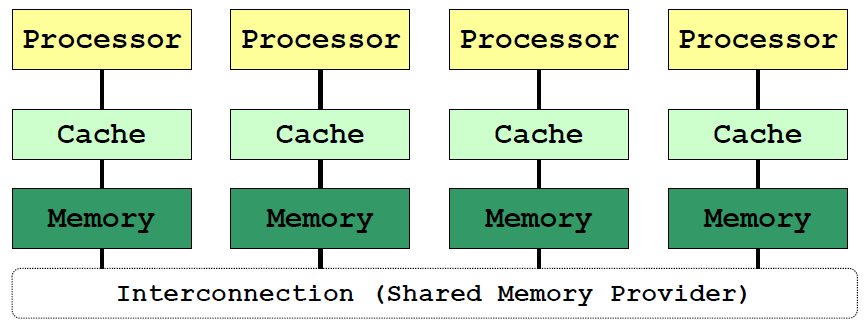
\includegraphics[width=0.9\textwidth]{l3_ccnuma.png}
              \item Cache Only Memory Architecture
                    \begin{itemize}
                        \item Each memory block works as cache memory
                        \item Uses cache coherence scheme to migrate datq
                    \end{itemize}
                    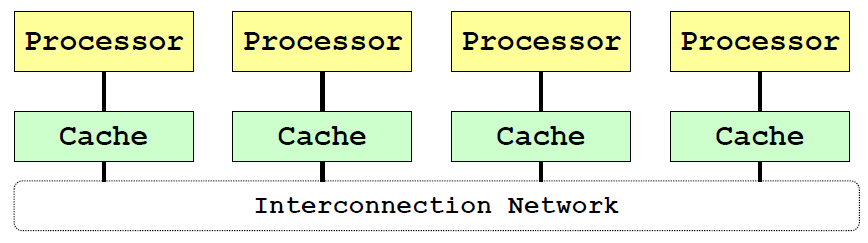
\includegraphics[width=0.9\textwidth]{l3_coma.png}
              \item Advantages
                    \begin{itemize}
                        \item No need to partition code or data
                        \item No need to physically move data among processors, there is effficient communication
                    \end{itemize}
              \item Disadvantages
                    \begin{itemize}
                        \item Special synchronization constructs are required
                        \item Lack of scalability due to contention
                    \end{itemize}
          \end{itemize}
    \item Hybird
          \begin{itemize}
              \item Servers, use shared among distributed
          \end{itemize}
\end{itemize}

\section{Chapter 4}
\subsection{Parallelism}
\textbf{Parallelism}: Average number of units of work that can be performed in parallel per unit time. MIPS, MFLOPS, etc.

Types of parallelism:
\begin{itemize}
    \item Data Parallelism
          \begin{itemize}
              \item Partition the data, each processing unit carries out similar operations on corresponding part of the data
              \item If operations are independent, elements can be distributed among processors for parallel execution.
              \item ex: SIMD, loop Parallelism if iterations are independent. (OpenMP)
              \item SPMD (single program Multiple Data): One parallel program is executed by all processorts in parallel (both shared and distributed address space)
          \end{itemize}
    \item Task Parallelism
          \begin{itemize}
              \item Partition the tasks, each processing unit handles one task
              \item A task can be one statement, loop, any number of statements or function calls
              \item A single task can be further decomposed. to be executed sequentially by one processor or in parallel by multiple processors.
              \item Example: in database query, different subqueries(different tasks) handled by different thread, then joined.
          \end{itemize}
\end{itemize}

\subsection{Models of Coordination}
How do our processes communicate?
\begin{itemize}
    \item Shared address space
          \begin{itemize}
              \item Tasks communicate by reading/writing to shared variables
              \item Ensure mutual exclusion via locks
              \item Required hardware support. (any processor can load and store from any address - contention, costly to scale)
              \item Very little structure, all threads can read and write to shared variable
              \item Drawback: not all read and writes have the same cost
          \end{itemize}
    \item Data parallel
          \begin{itemize}
              \item Historically: Same operation on different element of an array (SIMD, vector processors)
              \item No communication among distinct function calls, side-effect free execution
              \item Model performance-oriented data-parallel languages do not strictly enforce this structure (CUDE, OpenCL, ISPC)
              \item Very rigid computation structure
          \end{itemize}
    \item Message passing
          \begin{itemize}
              \item Tasks operate within their won private address spaces, communicate by explicitly sending / receiving messages.
              \item MPI(Message Passing Interface), popular library
              \item Imagine 2 servers, sending data through internet to each other. Similar to distributed memory systems.
              \item Highly structured communication, all communication in the form of messages
          \end{itemize}
\end{itemize}

\subsection{Program Prallelization}
\begin{enumerate}
    \item Partitioning
          \begin{itemize}
              \item Partition a problem into many smaller pieces or tasks
              \item Divide computaion and data into independent pieces to maximize parallelism
          \end{itemize}
    \item Communication
          \begin{itemize}
              \item Provides data required by partitioned tasks (cost of paralleism)
              \item Deterine how tasks should commuinicate with one another.
              \item Local communication: Tasks need data from some number of other tasks (neighbors)
              \item Glocal communication: Don't create channels to contribute to final data early (don't have all threads add the same value, every few thread join, then join the joined)
          \end{itemize}
    \item Agglomeration
          \begin{itemize}
              \item Decrease communication and development costs, while maintaining flexibility
              \item Improve performance, maintain scalability, reduce communication overhead.
              \item reduce granularity,
          \end{itemize}
    \item Mapping
          \begin{itemize}
              \item Map tasks to processor (coress) to minimize total execution time
              \item Maximize processor utilization, (place task on different processor)
              \item minimize inter-processor communication (place tasks that communicate on same processor, contradiction above)
              \item OS does this, or Users in distributed memory systems
          \end{itemize}
\end{enumerate}

Simplified Version:
\begin{itemize}
    \item Decomposition of the computation (step 1 and 2)
    \item Scheduling (assignment of tasks to processes or threads) (step 3)
    \item Mapping of processes (or threads) to physical processors (or cores)
\end{itemize}
There existys parallelizing compilers the perform decomposition and scheduling.
But the dependence analysis is difficult for pointer-based computations or indirect addresssing.
Hard to predict at compile time, values known at run time.

\subsection{Paralle Programming Patterns}
Design pattern, but for parallel programming not software engineering
\begin{itemize}
    \item Fork-Join
          \begin{itemize}
              \item Create a child with fork, wait for termination (join)
              \item Pthreads, OpenMP, MPI
          \end{itemize}
    \item Parbegin-Parend
          \begin{itemize}
              \item Specify region with parbegin-parend construct, when reach this construct a set of threads are created and the statements are assigned to threads for execution
              \item Statements after this construct only run after all threads have finished
              \item OpenMP or compiler directives
          \end{itemize}
    \item SPMD
          \begin{itemize}
              \item Same program run on different processors but operate on different data.
              \item Different threads can execute different part of program (if-else bloock, different speed)
              \item User needs to determine synchronization.
          \end{itemize}
    \item SIMD
    \item Master-Worker (Master-Slave)
          \begin{itemize}
              \item A single program (master) controls execution flow of the program (coordination and initializations, I/O)
              \item Assigns work to worker threads to perform computation (wait for instructions)
          \end{itemize}
    \item Client-Server
          \begin{itemize}
              \item MPMD (Multiple Program Multiple Data) model
              \item Server compute requests from multiple clients concurrently.
              \item can have multiple threads to handle one request.
          \end{itemize}
    \item Pipelining
    \item Task pool
          \begin{itemize}
              \item A common data structure from which threads can access to retrieve tasks for execution
              \item Fixed number of threads. statically created by main thread.
              \item A thread generates thread, add to task pool
          \end{itemize}
    \item Producer-Consumer
\end{itemize}

\section{Performance}
\begin{itemize}
    \item Users want to reduce response time
    \item Computer managers want to have high thoughput
\end{itemize}
Response time of a program A includes:
\begin{enumerate}
    \item User CPU time: time CPU spends for executing program
    \item System CPU time:time CPU spends executing OS routines
    \item Waiting time: I/O waiting time and the execution of other programs because of time sharing
\end{enumerate}

\textbf{User CPU Time}

Depends on the instructions generated by compiler when translating program and execution time of each instruction.

\[
    Time_{\text{user}} \left( A \right) = N_{\text{cycle}} \left( A \right) \times Time_{\text{cycle}}
\]
\begin{center}
    \begin{tabular}{ |c|c| }
        \hline
        $Time_{\text{user}} \left( A \right)$ & User CPU time of a program A                                        \\
        \hline
        $N_{\text{cycle}}$                    & Total number of CPU cycles needed for all instructions              \\
        \hline
        $Time_{\text{cycle}}$                 & Cyckle time of CPU (clcok cycle time $\frac{1}{\text{clock rate}}$) \\
        \hline
    \end{tabular}
\end{center}

But each instruction has different execution time. Consider each time instruction $i$ differently.
\[
    N_\text{cycle} \left( A \right) = \Sigma_{i=1}^n n_i \left( A \right) \times CPI_i
\]
\begin{center}
    \begin{tabular}{ |c|c| }
        \hline
        $n_i \left( A \right)$ & number of isntruction of time $I_i$                               \\
        \hline
        $CPI_i$                & average number of CPU cycles needed for instruction of type $I_i$ \\
        \hline
        $N_{\text{cycle}}$     & Total number of CPU cycles needed for all instructions            \\
        \hline
    \end{tabular}
\end{center}
Thus if we use CPI
\[
    Time_\text{user}\left( A \right) = N_\text{instr} \left( A \right) \times CPI(A) \times Time_\text{cycle}
\]
\begin{center}
    \begin{tabular}{ |c|c| }
        \hline
        $Time_\text{user}\left( A \right)$ & User CPU time of a program                                                         \\
        \hline
        $N_\text{instr} \left( A \right)$  & Total number of instructions executed for A. Depends on architecture, and compiler \\
        \hline
        $CPI(A)$                           & Average Cycles per instruction. Depends on CPU, memory, compiler                   \\
        \hline
        $Time_\text{cycle}$                & Time per cycle                                                                     \\
        \hline
    \end{tabular}
\end{center}

If we incluude \textbf{Memory Access Time}
\[
    Time_\text{user}\left( A \right) = \left( N_\text{instr} \left( A \right)  \times CPI \left( A \right) + N_\text{rw\_op} \left( A \right) \times R_\text{miss} \left( A \right) \times N_\text{miss\_cycles} \right) \times Time_\text{cycle}
\]
\begin{center}
    \begin{tabular}{ |c|c| }
        \hline
        $N_\text{rw\_op} \left( A \right)$ & total number of read or write operation                         \\
        \hline
        $R_\text{miss} \left( A \right)$   & (read and write) miss rate                                      \\
        \hline
        $N_\text{miss\_cycles}$            & number of additional cycles needed for leading a new cache line \\
        \hline
    \end{tabular}
\end{center}

If we only consider reading time
\[
    T_\text{read\_access} \left( A \right) = T_\text{read\_hit} + R_\text{read\_miss} \left( A \right) \times T_\text{read\_miss}
\]
\begin{center}
    \begin{tabular}{ |c|c| }
        \hline
        $T_\text{read\_access} \left( A \right)$ & average read access time of a program A                         \\
        \hline
        $T_\text{read\_hit}$                     & time for a read access to the cache irrespective of hit or miss \\
        \hline
        $R_\text{read\_miss} \left( A \right)$   & cahce read miss rate of a program A                             \\
        \hline
        $T_\text{read\_miss}$                    & read miss penalty time                                          \\
        \hline
    \end{tabular}
\end{center}

We can expand memory access time to consider different level of cache
\[
    T_\text{read\_access} \left( A \right) = T^\text{L1}_\text{read\_hit} + R^\text{L1}_\text{read\_miss} \left( A \right) \times T^\text{L1}_\text{read\_miss}
\]
\[
    T^\text{L1}_\text{read\_access} \left( A \right) = T^\text{L2}_\text{read\_hit} + R^\text{L2}_\text{read\_miss} \left( A \right) \times T^\text{L2}_\text{read\_miss}
\]
In the end the global miss rate is $R^\text{L1}_\text{read\_miss} \left( A \right) \times R^\text{L2}_\text{read\_miss} \left( A \right)$

How to evaluate \textbf{throughput}

Million-Instruction-Per-Second (MIPS)
\[
    MIPS \left( A \right) = \frac{N_\text{instr} \left( A \right)}{Time_\text{user} \left( A \right) \times 10^6}
\]
\[
    MIPS \left( A \right) = \frac{\text{clock\_frequency}}{CPI \left( A \right) \times 10^6}
\]
But we can easily manipulate, a lot of short instruction vs low number of long instruction

Million-Floaring point-Operation-Per-Second (MFLOPS)
\[
    MFLOPS \left( A \right) = \frac{N_\text{fl\_ops} \left( A \right)}{Time_\text{user} \left( A \right) \times 10^6}
\]
\begin{itemize}
    \item $N_\text{fl\_ops} \left( A \right)$: number of floating point operations in program A
    \item But we do not differentiate between different types of floating point operation.
\end{itemize}

\subsection{Speedup}
We denote $T_p \left( n \right)$ as $T$ the time of the parallel program on all processors on $p$ processors for a problem of size $n$.
This contains everything, waiting time, time for computation, time for synchronization, exchange of data.

The cost of a paralle program with input size $n$ executed on $p$ processors: $C_[ \left( n \right) = p \times T_p \left( n \right)]$
We measuer the total amout of work performed by all processors $C_p\left( n \right)$.
A parallel program is cost-optimal if it executes the same total number of operation as the fastest sequential program.

We measure speed up with $S_p \left( n \right) = \frac{T_\text{best\_seq} \left( n \right)}{T_p \left( n \right)}$
In theory $S_p \left( n \right) \leq p$ always holds,
but in practice $S_p \left( n \right) > p$ can happen, ex: if problem working task fits in the cache.
One issue is that we do not know what is the best sequential algorithm. best order of growth or lowest execution time. Also difficulty of implementaion

The Parallel Program Efficiency is the actual degree of speedup performance acheived comapred to the maximum

\[
    E_p \left( n \right) = \frac{T_\text{best\_seq} \left( n \right)}{p \times T_p \left( n \right)}
\]
Ideal speedup $S_p\left( n \right) = p$, and idealy $S_p \left( n \right) = 1$
But if we space the problem, need to bnalance overhead, computation, locality of data. Small problem size has large overhead. Large program has a lot of trashing on disk.

\textbf{Amdahl's Law (1967)}
Speedup of parallel execution is limited by the fraction of the algorithm that cannot be parallelized (f).
\begin{itemize}
    \item $f \left( 0 \leq f \leq 1 \right)$ is called the sequential fraction.
    \item Also known as fixed-workload performance
\end{itemize}
But Amdahl's Law can be circumvented for large problem size! $f$ is not a constant, dependent on problem size.
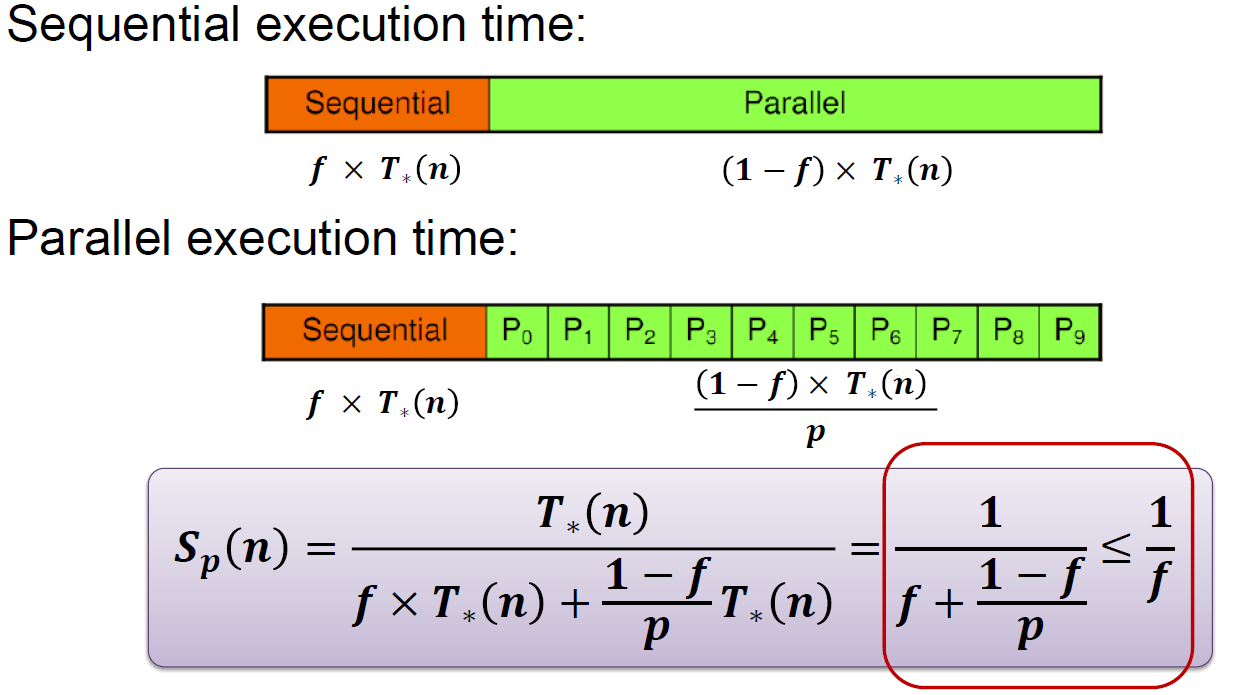
\includegraphics[width=0.8\textwidth]{l5_amdahl_law.png}

\textbf{Gustafson's Law (1988)}
There are certain applications where the main constaint is execution time.
if $f$ is not a constant but decreases when probelm size increases then $S_p \left( n \right) \leq p$

\section{GPGPU}
General Purpose GPU definitions:
\begin{itemize}
    \item Device: GPU
    \item Host: CPU
    \item Kernel: function that runs on the device
\end{itemize}
A GPU has Multiple Streaming Multiprocessors (SMs).
Each has memory and cache. one SM has multiple compute cores.

In a GPU, threads are very lightweight, very little overhead for creation, instant switching.


A CUDA kernel is executed by an array of threads. All threads run the same code, SPMD (Single Program, Multiple Data).
Each thread has an ID that it uses to compute memory addresses and make control decisions.
The threads need not be completely independent.

Threads are grouped up into blocks.
In a block, it has shared memory, atomic operations and barrier synchronization.
Threads in different blocks cannot cooperate.
We can scale to any number of processor by increasing blocks.
Hardware is free to schedule thread blocks to any processor at any time.
Kernel scales across any number of parallel multiprocessors.

Each thread uses IDs to decide what data to work on.
Can access block ID (1/2/3D), as well as thread ID.
Users can specify organization of block and threads(1/2/3D)

A kernel is executed by a grid of thread blocks.

A block executes on one streaming multiprocessor.
Does not migrate.
Several blocks can reside concurrently on one SM.
This is limited by SM resources.

Multiprocessor creates and manages, schedules and executes threads in SIMT warps(group of 32 parallel threads).
Threads in a warp start together at the same program address. Each thread has individual instruction program counter and register state.
A block is always split into warps the same way, a warp is consecutive threads in increasing IDs.
In one warp, only one common instructuion is done in all threads.
Avoid branching.



\subsection{CUDA Memory Model}
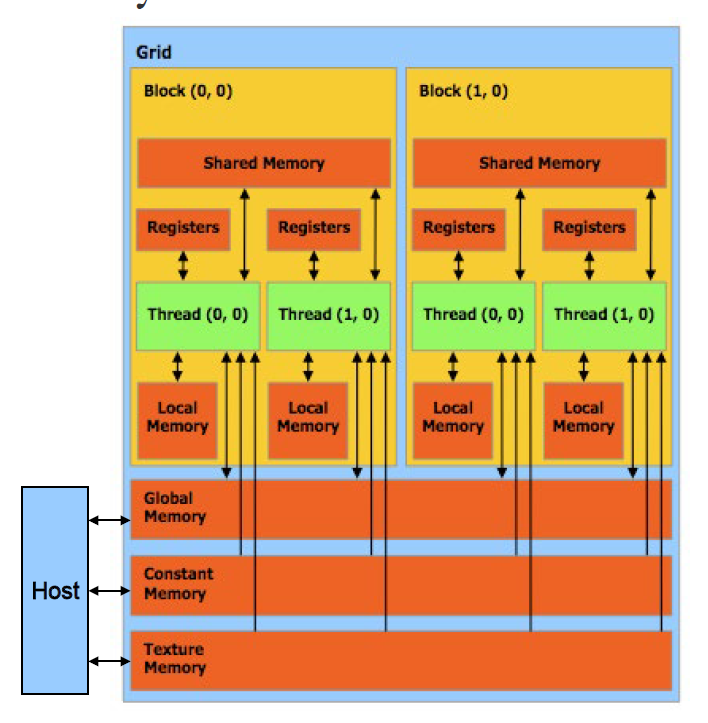
\includegraphics[width=0.9\textwidth]{l6_cuda_memory_model.png}

\begin{center}
    \begin{tabular}{| c | c| c | c| c| c| }
        \hline
        Type     & Scope   & Access type & Soeed    & CUDA declaration syntax  & Explicit sync \\
        \hline
        \hline
        register & thread  & RW          & fastest  & -                        & no            \\
        \hline
        Local    & thread  & RW          & depends* & float x                  & no            \\
        \hline
        Shared   & block   & RW          & fast     & \_\_shared\_\_ float x   & yes           \\
        \hline
        Glocal   & program & RW          & slow     & \_\_device\_\_ float x   & yes           \\
        \hline
        Constant & program & R           & slow     & \_\_constant\_\_ float x & yes           \\
        \hline
        Texture  & program & R           & slow     & \_\_texture\_\_ float x  & yes           \\
        \hline
    \end{tabular}
\end{center}
\begin{itemize}
    \item Local memory is actually an abstraction of global memory that is private to the thread.  So it is slower than shared memory.
    \item Shared memory has higher bandwidth, and lower latency than global and local memory. It is divided into equally sized momory modules, banks. Different addresses from different banks can be accessed simultaneously. if in the same bank, need to be serialized.
    \item Constant memory is useful for uniformly-accessed read-only data. It is cached
    \item Texture memory is useful for spatially coherent random-access read only data. It is cached. Provides filtering, address clamping and wrapping.
    \item simultaneous accesses to global memory by threads in a half-warp (16 threads) can be coalesced into as few as a single meory transaction of 32 / 64 / 128 bytes.
          \begin{itemize}
              \item when accessing global memory, it is 32 / 64 / 128 consecutive bytes segments are accessed together at one time.
              \item If all lie in the same region, one memory access, else need multiple transactions
          \end{itemize}
\end{itemize}

\section{Cache Coherence and Memory Consistency}
\subsection{Cache Coherence}
Cache is used to reduce memory access latency.

\begin{itemize}
    \item *Cache Size*: larger cache increases access time, increased addressing complexity. but reduces cache misses
    \item *Block Size*: data is transferred between main memory and cache in blocks of fixed length
          \begin{itemize}
              \item Larger blocks reduce number of block but replacements take longer
              \item Larger block increases probability of spacial locality
          \end{itemize}
\end{itemize}

How do we write to cache and memory:
\begin{itemize}
    \item Write-Through
          \begin{itemize}
              \item write access is immediately transferredto main memory
              \item Advantage: always gets neweest value of a memory block
              \item Disadvantage: slow down due to many memory access (use write buffer)
          \end{itemize}
    \item Write-Back
          \begin{itemize}
              \item write operation is only on cache, written to main memory when cache block is replaced. Uses a dirty bit.
              \item Advantage: uses less write operations
              \item Disadvantage: Memory has invalid entries
          \end{itemize}
\end{itemize}

\textbf{Cache Coherence} problem is when multiple entries of the same data exists on different cache.
One processor updates the data, other processors may still see unchanged data.
Issue arrises because we have one global memory, and many local memory.

\subsubsection{Memory Coherence}
Three properties of memory Coherence
\begin{itemize}
    \item \textbf{Program Order}
          \begin{itemize}
              \item Given the sequence
                    \begin{enumerate}
                        \item $p$ write to \textbf{x}
                        \item No more writes to \textbf{x}
                        \item $p$ reads from \textbf{x}
                    \end{enumerate}
              \item $p$ should get the value written in step 1
          \end{itemize}
    \item \textbf{Write Propagation}
          \begin{itemize}
              \item Given the sequence
                    \begin{enumerate}
                        \item $p_1$ write to \textbf{x}
                        \item No more writes to \textbf{x}
                        \item $p_2$ reads from \textbf{x}
                    \end{enumerate}
              \item $p_2$ should read value written in by $p_1$
              \item Writes become visible to other processors
          \end{itemize}
    \item \textbf{Write Serialization}
          \begin{itemize}
              \item Given the sequence
                    \begin{enumerate}
                        \item write $v_1$ to \textbf{x}, by any processor
                        \item write $v_2$ to \textbf{x}, by any processor
                    \end{enumerate}
              \item any processor can never read \textbf{x} as $v_2$ and then later $v_1$
              \item ALl writes to the same location (from same or different processors) are seen in the same order by all processors
          \end{itemize}
\end{itemize}

Cache coherence can be solved using
\begin{itemize}
    \item Software Based Solution
          \begin{itemize}
              \item OS + compiler + Hardware aided solution
          \end{itemize}
    \item Hardware Based Solution
          \begin{itemize}
              \item Most common on multiprocessor system
              \item Known as cache coherence protocols
          \end{itemize}
\end{itemize}

Major tasks for Hardware Cache Coherence Protocols:
\begin{itemize}
    \item Track the sharing status of a cache line
    \item Handle the update to a shared cache line
\end{itemize}

There are 2 major catagories of solutions:
\begin{itemize}
    \item Snooping based:
          \begin{itemize}
              \item No centralized directory
              \item Each cache monitors or snoop on the bus, to update status  of cache line and take appropiate action
              \item Most common protocol used in architecture with a bus
          \end{itemize}
    \item Directory based:
          \begin{itemize}
              \item Sharing status is kept in a centralized location
              \item commonly used with NUMA architectures
          \end{itemize}
\end{itemize}

Bus based cache coherence:
\begin{itemize}
    \item All the processors on the bus can observe every bus transaction, *Write Porpagation*
    \item Bus transaction are visible to the processors in the same order, *Write Serialization*
\end{itemize}
The cache controllers "snoop" on the bus and monitor transactions, takes relevant actions.
Some issues that arrise due to cache coherence:
\begin{itemize}
    \item Overhead in shared address space:
          \begin{itemize}
              \item Cache Coherence appears as increased memory latency in multiprocessor
              \item Cache Coherence lowers the hit rate in cache
          \end{itemize}
    \item False Sharing
          \begin{itemize}
              \item 2 processors write to different address in the same cache line
          \end{itemize}
\end{itemize}

\subsection{Memory Consistency Models}
4 types of memory operation ordering:
\begin{enumerate}
    \item $W \rightarrow R$
    \item $R \rightarrow R$
    \item $R \rightarrow W$
    \item $W \rightarrow W$
\end{enumerate}

These 4 need not be preserved.
We can relax some restrictions, Relax consistencies, to hide write latencies.
If there is no data dependency in one processor.

Some memory models:
\begin{itemize}
    \item Sequential Consistency \textit{SC}
          \begin{itemize}
              \item Every processor issues its memory operations in program order
              \item Extension of uniprocessor memory model, intuitive but can have loss in performance
              \item As if one memory space, ne memory operation at one time
          \end{itemize}
    \item Total Store Ordering \textit{TSO}
          \begin{itemize}
              \item Return the value written by $P$ ealier without waiting for it to be serialized
              \item Relaxes $W \rightarrow R$
              \item Does not ensure *Write Serialization*
              \item Data dependencies in one program must be preserved!
          \end{itemize}
    \item Processor Consistency - \textit{PC}
          \begin{itemize}
              \item Return the value of any write (even from another processor) before the write is propagated or serialized
              \item Relaxes $W \rightarrow R$
              \item Does not ensure *Write Serialization* and *Write Propagation*
              \item Data dependencies in one program must be preserved!
          \end{itemize}
    \item Partial Store Order - \textit{PSO}
          \begin{itemize}
              \item Write can bypass earlier writes (to different locations) in write buffer. Allows write miss to overlap and hide latency
              \item Relaxes $W \rightarrow R$, similar to TSO, and $W \rightarrow W$
              \item Data dependencies in one program must be preserved!
          \end{itemize}
\end{itemize}
The last 3 above are relaxed consistencies.

\section{Parallel Programming Models - II}
\subsection{Data Distribution}
There are many ways to distribute data on multiple processors.
Known as data distribution / work distribution / decomposition / partitioning.
Problems that exhibit data parallelism, data distribution can be used as a simple parallization strategy.
Commonly distributed Blockwise or cyclic or some combination of the two.

\subsection{Information Exchange}
To communicate between different processes for coordination in a parallel process.
For Shared address space, usually used \textbf{shared variables}.
For distributed address space, use \textbf{communication operations}.

Shared memory programming models assume a global memory accessible by all processors.
programmer responsible to ensure safe concurrent access.
Each thread executed by one processor or core, have shared variables and may have private variables.
Uses critical section such as mutex.

In distributed memory programming we assume disjoint memory space.
Need to use dedicated communication operations.
one sends, one receives. known as message-passing programming model.
data exchanges can be point-to-point or global.
Data is explicitly partitioned into each process.
All interactions need both parties to participate.
Programmer needs to explicitly express parallelism.

Principles of Message Passing Model:
it is loosely synchronous paradigm.
Tasks or subsets of tasks synchronize to perform interactions.
between there interactions tasks execute completely asynchronous.

\subsection{Communication Protocol}
\subsubsection{Send and Receive Operations}
one process sends to another process.
In a distributed memory system, over a network. THis is a one way transfer.

\begin{tabularx}{0.8\textwidth} {
        | >{\raggedright\arraybackslash}X
        | >{\centering\arraybackslash}X
        | >{\raggedleft\arraybackslash}X |}
    \hline
                 & Blocking Operation                                                            & Non-Blocking Operation                                                                                                  \\
    \hline
    Buffered     & Sending process returns after data has been copied into communication buffer  & SendinSending process returns after initiating the transfer to buffer. This operation might not be completed on returng \\
    \hline
    Non-Buffered & Sending process blocks until matching receive operation has been encountered. &                                                                                                                         \\
    \hline
    Comments:    & Send and receives semantics assured by corresponding                          & Programmer must explicitly ensure completion of the operation by polling.                                               \\
    \hline
\end{tabularx}

In a blocking operation, send operation blocks until it is safe to reuse the input buffer.
"Safe" refers to the integrity of the data to be sent.

Non-buffered blocking send:
the operation blocks until the matching receive operation has been performed by receiveing process.
Can lead to idling and deadlocks.
There are idling overhead, waiting sender and receiver to be ready

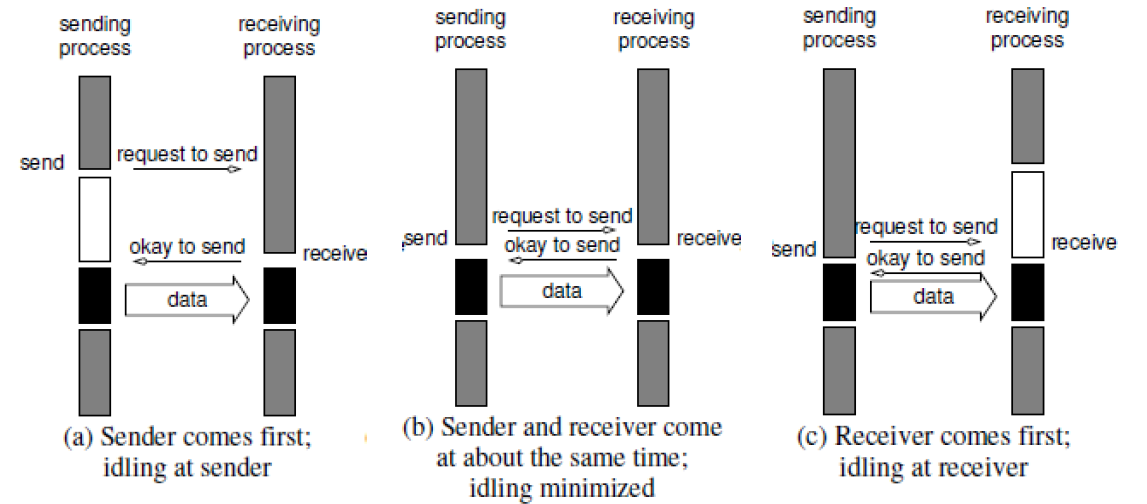
\includegraphics[width=0.9\textwidth]{l8_non_buffered_blocking.png}

To reduce the idling overhaed, we use buffers.
Send data to designated buffer and return after the copy operation has been completed.
Receiver similarly buffers the incoming data.
Buffering trades off idling overhead for buffer copying overhead.

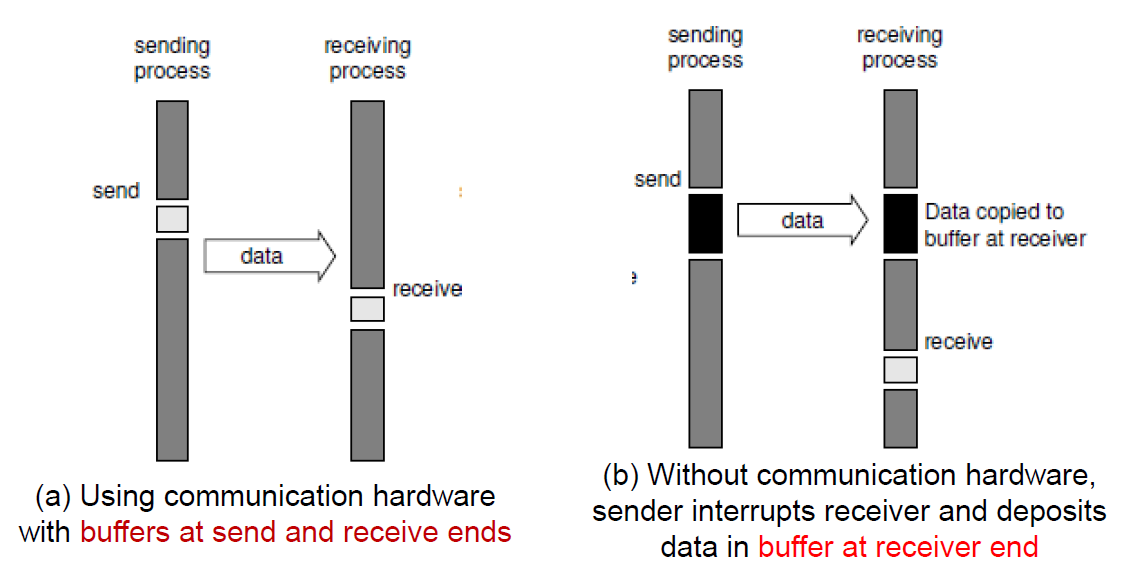
\includegraphics[width=0.9\textwidth]{l8_buffered_blocking.png}

In Non-blocking operation, Send/Receive returns before it is semantically safe to do so.
Non-blocking operations are generlly acompanied by a checking mechanism.
Programmer checks if it is safe to use data.
If used correctly, can overlap communication overhead.

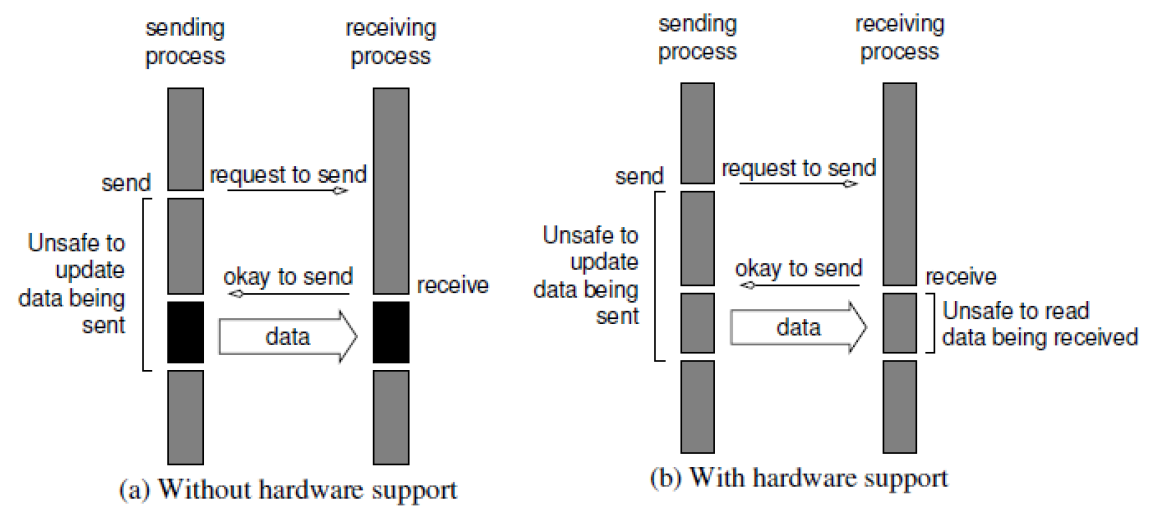
\includegraphics[width=0.9\textwidth]{l8_non_buffered_non_blocking.png}

Semantics of Send/Receive operations:

\begin{tabularx}{0.9\textwidth} {
        | >{\centering\arraybackslash}X
        | >{\centering\arraybackslash}X |}
    \hline
    Local view                                                                                                                                            & Global VIew \\
    \hline
    \textbf{Blocking}: Return from a library call indicates the user is allowed to reuse resources specified in the call                                  &
    \textbf{Synchronous} Communication operation does not complete before both processes have started their communication operation                                     \\
    \hline
    \textbf{Non-blocking}: A procedure may return before the operation completes, and before the user is allowed to reuse resources specified in the call &
    \textbf{Asynchronous}: Sender can execute its communication operation without any coordination with the receiver                                                    \\
    \hline
\end{tabularx}

\section{Message Passing}
Coding see lecture slides.

\subsection{Collective Communication}
There are many communicatoin operations: single tranfer, gather (scatter)
Typically is like this: sencer (root) sends to slave processeors to do work. then gather accumulate their results.
Processors are given an id / rank.
\begin{itemize}
    \item Single broadcast: Sender (root processor) sends the same data to all other processes.
    \item Multi broadcast: Each processor sends the same data block to every other processor. NO root processor. Data blocks are collected in rank order
    \item Single accumulation (Gather with reduction): Each processor provides a block of data with the same type and size. A reduction ( binary, associative and commutative ) operation is applied element by element to the data blocks. Root process receives result.
    \item Multi accumulation:  Each processor provides for every other processor a potentially different data block.Data blocks for the same receiver are combined with a given reduction operation. No root processor.
    \item Total Exchange: Each processor provides for each other processor a potentially different data block. Effectively each processor executes a scatter operation. No root processor
\end{itemize}

\section{Interconnection}

Interconnection network is cool.

\subsection{Topology}
What is the geometrical shape of the connection.

There are 2 major types of Topology:
\begin{itemize}
    \item Direct Interconnection
          \begin{itemize}
              \item Static or point-to-point
              \item endpoints are usually the same (core, memory)
          \end{itemize}
    \item Indirect Interconnection
          \begin{itemize}
              \item Dynamic
              \item Interconnect formed by switches
          \end{itemize}
\end{itemize}

We can model this as a graph. $G = \left( V, E \right)$, $V$ = vertices / node, $E$ = edges
We are concerned about:
\begin{itemize}
    \item Diameter $\delta \left( G \right)$
          \begin{itemize}
              \item Maximum distance between any pair of nodes
              \item small diameter ensures small distances for message transmission
          \end{itemize}
    \item Degree
          \begin{itemize}
              \item $g\left( v \right)$: number of direct neighbour nodes of a node $v$
              \item $g\left( G \right)$: maximum degree of a node in a network $G$
              \item small node degree reduces the node hardware overhead
          \end{itemize}
    \item Bisection Width $B \left( G \right)$
          \begin{itemize}
              \item minimum number of edges that must be removed to divide the network into 2 equal halves
              \item Bisection Bandwidth $BW\left( G \right)$: Total bandwidth available between the two bisected portion of the network.
              \item A measure for the capacity of a network when transmitting messages simultaneously
          \end{itemize}
    \item Connectivity
          \begin{itemize}
              \item Node Connectivity $nc \left( G \right)$: minimum number of nodes that must fail to disconnect the network.
              \item To determine the robustness of the network
              \item Edge Connectivity $ec \left( G \right) $: minimum number of edges that must fail to disconnect the network.
              \item Determine number of independent paths between any pair of nodes
          \end{itemize}
\end{itemize}

\subsection{Indirect Interconnection}
Reduce hardware cost by sharing switches and links.
Use switches to provide indirect connection between nodes and can be configured dynamically.
metrics to consider are cost / number of switch/link and concurrent connections.

\subsubsection{Bus network}
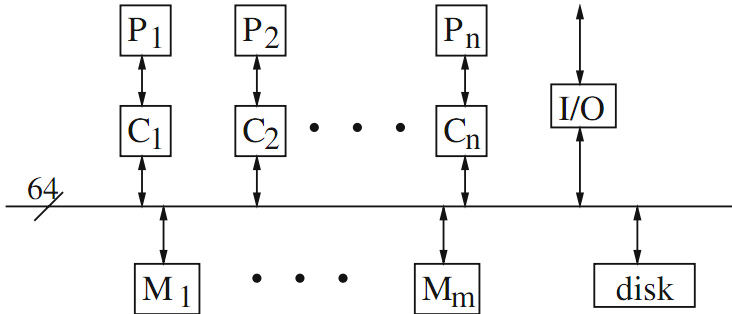
\includegraphics[width=0.9\textwidth]{l10_bus_network.png}

A set of wires to transport data from a sender to a receiver.
Only one pair of devices can communicate at a time.
A bus arbiter is used for the coordination.
Typically used for a small number of processors.

\subsubsection{Crossbar network}
A $n \times m$ crossbar network has $n$ inputs and $m$ outputs.

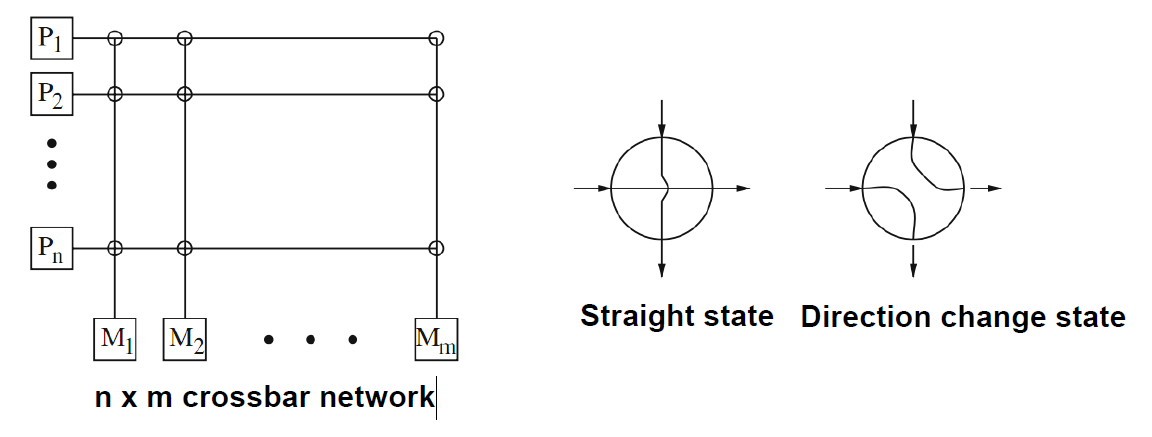
\includegraphics[width=0.9\textwidth]{l10_crossbar_network.png}

The switches can either be straight or direction change.
But it is expensive. $n \times m$ switches for few number of processors.

\subsection{Multistage Switching Network}
Several intermediate switches with connecting wires between neighbouring stages.
Goal: obtain a small distance for arbitraty pairs of input and output devices.
each switch has 2 input and 2 outputs.

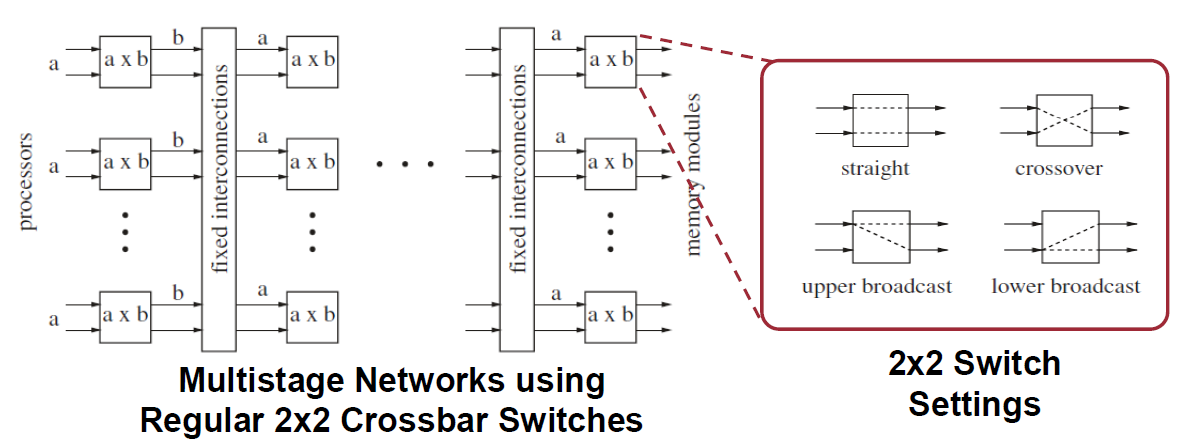
\includegraphics[width=0.9\textwidth]{l10_multistage_switching_network.png}

\subsection{Omega Network}

One unique path for every input to output
an $n \times n$ omega network has $\log n$ stages and $n/2$ switches per stage.
The connections between stages are regular. Also known as $\left( \log n - 1\right)$ - dimension Omega Network
\begin{itemize}
    \item A switch position $\left(\alpha , i\right)$, where $\alpha$ is the position of a stage within a stage; $i$: stage number
    \item Has an edge from node $\left(\alpha , i\right)$ to two nodes $\left(\beta, i + 1\right)$ where
          \begin{itemize}
              \item $\beta = \alpha$ by a cyclic left shift
              \item $\beta = \alpha$ by a cyclic left shift + inversion of the LSBit
          \end{itemize}
\end{itemize}

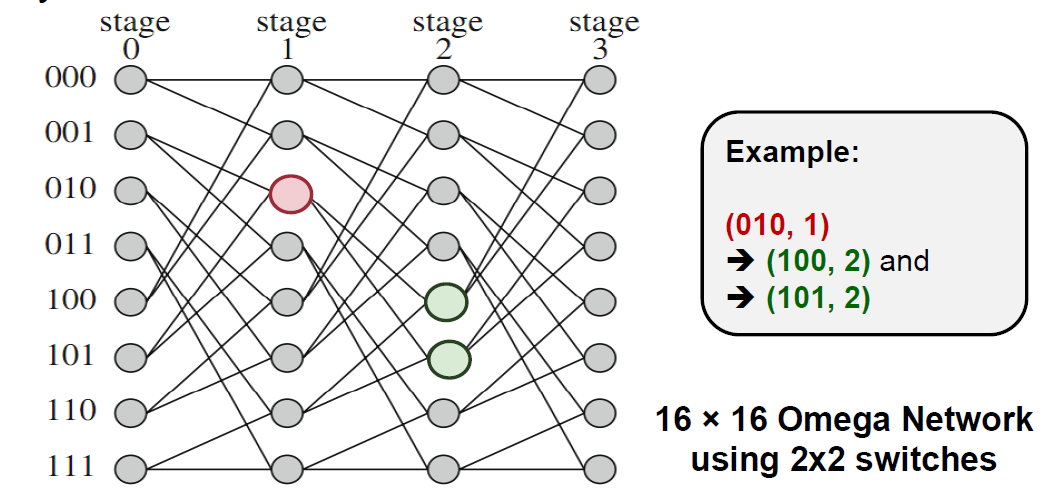
\includegraphics[width=0.9\textwidth]{l10_omega_network.png}

In a 16 processor to 16  memory nodes, crossbar needs $16 \times 15 = 256$ switches.
Omega needs $\log n \times n/2 = 4 * 8 = 32$ switches.

\subsection{Butterfly Network}
\begin{itemize}
    \item Node $\left( \alpha , i \right)$ connets to
          \begin{itemize}
              \item $\left( \alpha , i + 1 \right)$, i.e. straight edge
              \item $\left( \alpha^\prime , i + 1 \right)$, $\alpha$ and $\alpha^\prime$ differ in the $\left( i + 1 \right)$th bit from the left, i.e. cross edge
          \end{itemize}

\end{itemize}

\subsection{Baseline Network}
\begin{itemize}
    \item A switch position $\left(\alpha , i\right)$, where $\alpha$ is the position of a stage within a stage; $i$: stage number
    \item Has an edge from node $\left(\alpha , i\right)$ to two nodes $\left(\beta, i + 1\right)$ where
          \begin{itemize}
              \item $\beta =$ cyclic right shift of last $\left( k - i \right)$ bits of $\alpha$
              \item $\beta =$ inversion of the LSBit of $\alpha$ + cyclic right shift of last $\left( k - i \right)$ bits
          \end{itemize}
\end{itemize}

\subsection{Routing}
How to go from processor to memory.

Routing algorithms Classifications
\begin{itemize}
    \item Based on path length
          \begin{itemize}
              \item Minimal or Non-minimal routing: whether the shortest path is always chosen
          \end{itemize}
    \item Based on adapticity
          \begin{itemize}
              \item Deterministic: Always use the same path for the same pair of $\left( source, destination \right)$ node
              \item Adaptive: May take into account of network status and adapt accordingly, e.g. avoid congested path. Avoid dead nodes, etc.
          \end{itemize}
\end{itemize}

Some deterministic routing examples:
\begin{enumerate}
    \item XY routing for 2D Mesh
          \begin{itemize}
              \item $\left( X_{\text{src}}, Y_{\text{src}}\right)$ to $\left( X_{\text{dst}}, Y_{\text{dst}}\right)$
              \item Move in $X$ direction until $X_{\text{src}} == X_{\text{dst}}$
              \item Move in $Y$ direction until $Y_{\text{src}} == Y_{\text{dst}}$
          \end{itemize}
    \item E-Cube Routing for Hypercube
          \begin{itemize}
              \item Let $\left( \alpha_{n-1} \alpha_{n-2} \dots \alpha_0 \right)$ and $\left( \beta{n-1} \beta{n-2} \dots \beta\right)$ be the bit representations of source and destination node address respectively.
              \item Number of bits difference in source and target node address means number of hops, also known as hamming distance.
              \item Start from MSB to LSB (or LSB to MSB)
              \item Find the first different bit, go to the neighboring node with the bit corrected, at most $n$ hops.
          \end{itemize}
    \item XOR-Tag Routing for Omega Network
          \begin{itemize}
              \item Let $T = \text{Source Id} \oplus \text{Destination Id}$
              \item At stage-$k$:
                    \begin{itemize}
                        \item Go straight if bit $k$ of $T$ is 0
                        \item crossover if bit $k$ of $T$ is 1
                    \end{itemize}
          \end{itemize}
\end{enumerate}


\section{Definitions}
\textbf{Blocking call}: Control returns only when the call completes.

\textbf{Non blocking call}: Control returns immediately. Later OS somehow notifies the process that the call is complete.

\textbf{Synchronous program}: A program which uses Blocking calls. In order not to freeze during the call it must have 2 or more threads (that's why it's called Synchronous - threads are running synchronously).

\textbf{Asynchronous program}: A program which uses Non blocking calls. It can have only 1 thread and still remain interactive.

Concurrent and parallel are effectively the same principle as you correctly surmise, both are related to tasks being executed simultaneously although I would say that parallel tasks should be truly multitasking, executed "at the same time" whereas concurrent could mean that the tasks are sharing the execution thread while still appearing to be executing in parallel.

Asynchronous methods aren't directly related to the previous two concepts, asynchrony is used to present the impression of concurrent or parallel tasking but effectively an asynchronous method call is normally used for a process that needs to do work away from the current application and we don't want to wait and block our application awaiting the response.

\end{document}
